\section{The fixed shell and its three paired regions}\label{sec:shell}
\subsection{An exact coordinate realization}
Put $s=\sqrt2-1$, $d=1-\sqrt2/2$, $h_0=s/2$. In a panel's coordinates $(u,z)$ use the cyclic list
\begin{equation}\label{eq:octagon}
\begin{split}
(-\tfrac12,-h_0),\ (-h_0,-\tfrac12),\ (h_0,-\tfrac12),\ (\tfrac12,-h_0),\\
(\tfrac12,h_0),\ (h_0,\tfrac12),\ (-h_0,\tfrac12),\ (-\tfrac12,h_0).
\end{split}
\end{equation}
Let $D_8$ be their filled convex octagon. The three isometric embeddings are
\begin{equation}\label{eq:panels}
\begin{aligned}
f_1(u,z)&=(-\tfrac14-\tfrac u2,\ \tfrac{\sqrt3}4-\tfrac{\sqrt3}2u,\ z),\\
f_2(u,z)&=(u,0,z),\\
f_3(u,z)&=(\tfrac14-\tfrac u2,\ \tfrac{\sqrt3}4+\tfrac{\sqrt3}2u,\ z).
\end{aligned}
\end{equation}
The material shell is $S=f_1(D_8)\cup f_2(D_8)\cup f_3(D_8)$, with centre $O=(0,\sqrt3/6,0)$. Thus $S$ includes the entire panels, not only their edges. Equations \eqref{eq:octagon}--\eqref{eq:panels} reproduce Paper C's width-one realization without any project import.~\cite[Secs.~2--4]{PC}

The welded vertex numbering is fixed as follows. Traverse $f_1$ in the order \eqref{eq:octagon} and assign IDs $0,\ldots,7$. The $f_2$ cycle is $(3,8,9,10,11,12,13,4)$; the $f_3$ cycle is $(10,14,15,0,7,16,17,11)$. This is a complete coordinate prescription for all eighteen vertices, including each alias at a seam. The three seams are $(0,7),(3,4),(10,11)$.

\begin{proposition}[Inherited shell topology]\label{prop:topology}
The specified shell is a connected compact orientable surface with boundary, with eighteen vertices, twenty-one edges, three faces and two disjoint nine-edge boundary rims. It is an annulus.
\end{proposition}
\begin{proof}
We reuse Paper C, Section 5, Theorems 1 and 1b, with exactly the maps \eqref{eq:panels}. To make the inherited hypotheses visible: the three seams identify three pairs of edges and six pairs of vertices, giving $E=24-3=21$ and $V=24-6=18$. The face adjacency graph is connected. Each seam interior has two glued half-disc neighbourhoods; each free edge has one. Every vertex link is an interval: a single-panel corner gives one link edge, and a seam endpoint gives two joined link edges. The panel planes meet only along the prescribed seams within the panels. Opposite traversal of each seam by its adjacent face cycles gives orientation. Tracing the eighteen free edges gives one nine-edge cycle above $z=0$ and another below it. Consequently $\chi=18-21+3=0$ and $b=2$. The orientable-surface classification applied in the cited theorem gives $0=2-2g-2$, hence genus zero and the annulus type. A torus would instead have no boundary.
\end{proof}

\subsection{Finite measurement triangles}
Define
\begin{equation}\label{eq:axes}
r_0=1/\sqrt3,\quad c=\sqrt3/2,\quad
u_j=R_z(2\pi j/3)(0,1,0),\quad v_j=\ez\times u_j,
\end{equation}
where $j=0,1,2$ and $R_z$ is the ordinary right-handed rotation. The three seam footprints are $O+r_0u_j$. For $\sigma\in\{+1,-1\}$ set
\begin{equation}\label{eq:triangles}
\Delta_j^\sigma=\left\{O+(r_0-cdt)u_j+\xi v_j+\sigma(h_0+dt)\ez:
0\le t\le1,\ |\xi|\le dt/2\right\}.
\end{equation}
Here $t$ is a triangle coordinate only; analysis time will occur only in later sections. The two tip-to-base sides are material rim edges. The third side closes a measurement region between the two base vertices and adds no material panel or cap. The orientation and ID order are
\begin{center}
\begin{tabular}{@{}ccc@{}}\toprule
Pair & Upper, tip first & Lower, tip first\\\midrule
$P0$ & $(7,6,16)$ & $(0,15,1)$\\
$P1$ & $(4,13,5)$ & $(3,2,8)$\\
$P2$ & $(11,17,12)$ & $(10,9,14)$\\\bottomrule
\end{tabular}
\end{center}
These triangles describe three paired geometric regions, not six additional boundary components. In particular, their shared upper/lower projected footprints are not an identification of their spatial points.

\begin{proposition}[Planes, normals and contacts]\label{prop:contacts}
The oriented unit normals and supporting planes of \eqref{eq:triangles} are
\begin{equation}\label{eq:planes}
n_j^\sigma=\frac{2u_j+\sigma\sqrt3\ez}{\sqrt7},\qquad
u_j\cdot(X-O)+\sigma cX_z=\kk,\quad
\kk=\frac{\sqrt3}{12}+\frac{\sqrt6}{4}.
\end{equation}
Let $a=\kk/(1+c)$. The selected median points
\begin{equation}\label{eq:contacts}
P_j^\pm=O+a u_j\pm a\ez,\qquad t_0=(a-h_0)/d
\end{equation}
belong to the relative interiors of their triangles, with tip-first barycentric coordinates $(1-t_0,t_0/2,t_0/2)$.
\end{proposition}
\begin{proof}
Substitution in the left side of \eqref{eq:planes} gives $r_0-cdt+c(h_0+dt)=r_0+ch_0=\kk$. The two tangent directions $v_j$ and $-c u_j+\sigma\ez$ are perpendicular to the stated unit normal; the printed vertex orders give its sign. At $P_j^\sigma$, the plane equation is $a(1+c)=\kk$ and the transverse coordinate is zero. Also
\[
a-h_0=\frac{r_0-h_0}{1+c}>0,\qquad
\tfrac12-a=\frac{(1+c)/2-\kk}{1+c}>0.
\]
For explicit inequalities, $h_0<1/4<r_0$ follows from $\sqrt2<3/2$ and $\sqrt3<2$; and $(1+c)/2-\kk=1/2+\sqrt3/6-\sqrt6/4>0$, since $\sqrt3>3/2$ and $\sqrt6<5/2$ give a lower bound $1/8$. Since $h_0+d=1/2$, we have $0<t_0<1$. The triangle is the affine interpolation between its tip and its base segment, so the displayed barycentrics follow and are strictly positive.
\end{proof}

Numerically, $\kk\simeq0.756710$, $a\simeq0.405520$, and $t_0\simeq0.677424$. These values are consequences of the specified planes. The contacts are not triangle centroids. Their selection is the median member of the recovered Gate/Torus contact family, not a fit to any unrelated constant.~\cite[Sec.~3.3]{Gate}

\section{A conditional normal-crossing circle}\label{sec:circle}
We now make the added geometric choice explicit: seek a Euclidean circle in the affine median plane $O+\operatorname{span}(u_j,\ez)$, through $P_j^+$ and $P_j^-$, with tangent parallel to the relevant patch normal at each contact. This is one precise version of the transverse-loop picture. Its uniqueness is relative to this family.

\begin{theorem}[Selected circle and finite crossings]\label{thm:circle}
There is exactly one circle with those properties. Its centre, radius and oriented parametrization are
\begin{equation}\label{eq:circle}
B_j=O+\kk u_j,\quad R_\Gamma=\frac{\sqrt7}2a,\quad
\Gamma_j(\chi)=B_j+R_\Gamma(\cos\chi\,u_j+\sin\chi\,\ez).
\end{equation}
It meets each of its two finite measurement triangles exactly once, at $P_j^\sigma$, with unit tangents $-n_j^+$ above and $+n_j^-$ below. It meets none of the other four triangles.
\end{theorem}
\begin{proof}
Equal distances from a planar centre $O+b u_j+z_b\ez$ to $P_j^+$ and $P_j^-$ give $4az_b=0$, hence $z_b=0$. Orthogonality of the upper contact radius to the prescribed normal then requires
\[
0=(P_j^+-B_j)\cdot n_j^+
=\frac{2(a-b)+\sqrt3a}{\sqrt7}.
\]
Thus $b=(1+c)a=\kk$ and the radius squared is $(a-\kk)^2+a^2=(1+c^2)a^2=7a^2/4$. The lower condition gives the same equation. These deductions are necessary and, by substitution, sufficient, proving uniqueness.

At the contacts, $\cos\chi=-\sqrt{3/7}$ and $\sin\chi=\sigma2/\sqrt7$. Differentiating \eqref{eq:circle} gives the stated unit tangents. The supporting plane cuts the circle in a line through $B_j$ because $u_j\cdot(B_j-O)=\kk$. Its two intersections are therefore $P_j^\sigma$ and $2B_j-P_j^\sigma$. The latter has height $-\sigma a$, whereas every point of $\Delta_j^\sigma$ has height of sign $\sigma$. Only the first intersection belongs to the finite triangle. Proposition~\ref{prop:contacts} proves its interior membership, and the nonzero normal derivative proves transversality.

For $\ell\ne j$, a point of $\Delta_\ell^\sigma$ has $u_j$ projection at most
\[
-\tfrac12(r_0-cdt)+\tfrac{\sqrt3}{2}\tfrac{dt}{2}
=-r_0/2+cdt\le-r_0/2+cd<0.
\]
The last inequality is $d<1/3$, which follows from $\sqrt2>4/3$. The circle's projection is at least $\kk-R_\Gamma>0$, because $1+c>\sqrt7/2$. It cannot reach another pair.
\end{proof}

The right-angle operation has a definite pivot and order. Start with the horizontal parent circle $B_j+R_\Gamma(\cos\chi\,u_j+\sin\chi\,v_j)$ and rotate by $+\pi/2$ about the radial line through $O$ and $B_j$, using $B_j$ as pivot. This sends $v_j$ to $\ez$ and $\ez$ to $-v_j$. The resulting circle's axis is $-v_j$, perpendicular to the central shell axis. The shell itself is not rotated by this operation.

\begin{theorem}[Whole-circle clearance and the planar obstruction]\label{thm:clearance}
Each $\Gamma_j$ is disjoint from the filled shell $S$. The three circles are mutually disjoint, with pairwise distance at least $\sqrt3(\kk-R_\Gamma)>0$. No plane, hence no planar circle, contains all six selected contacts.
\end{theorem}
\begin{proof}
Work in a fixed median plane and write $X-O=r u_j+z\ez$. The opposite panel has meridian section $r=-1/(2\sqrt3)$. Since $r\ge\kk-R_\Gamma>0$ on the circle, that panel is excluded. The remaining two panel planes meet this median plane only on their common seam line $r=r_0$; their material portions there satisfy $|z|\le h_0$. The circle instead has, at that line,
\begin{equation}\label{eq:seamclear}
z^2=R_\Gamma^2-(r_0-\kk)^2
=\frac{113}{6}+\frac{13\sqrt2}{2}-\frac{133\sqrt3}{12}-\frac{7\sqrt6}{2}>\frac14>h_0^2.
\end{equation}
For a fully explicit certificate of the close first inequality, use the rational enclosures
\[
\begin{array}{c}
1.41421356237<\sqrt2<1.41421356238,\\
1.73205080756<\sqrt3<1.73205080757,\\
2.44948974278<\sqrt6<2.44948974279.
\end{array}
\]
Each follows by squaring positive rational endpoints. Substitution of lower endpoints in positive terms and upper endpoints in negative terms gives a rational lower bound greater than $0.2556109383$, itself greater than $1/4$. The second inequality follows from $h_0<1/4$. This covers panel interiors as well as edges, without sampling the circle.

For two different median planes, points of the circles have horizontal projections $r u_j$ and $r' u_\ell$, with $r,r'\ge m:=\kk-R_\Gamma>0$. Since $u_j\cdot u_\ell=-1/2$, their squared horizontal distance is $r^2+r'^2+rr'\ge3m^2$. Vertical differences only increase total distance. Finally, the three upper contacts form a nondegenerate triangle in $z=a$; they determine that plane. No lower contact with $z=-a$ lies in it. This proves the planar obstruction.
\end{proof}

\begin{figure}[htbp]\centering
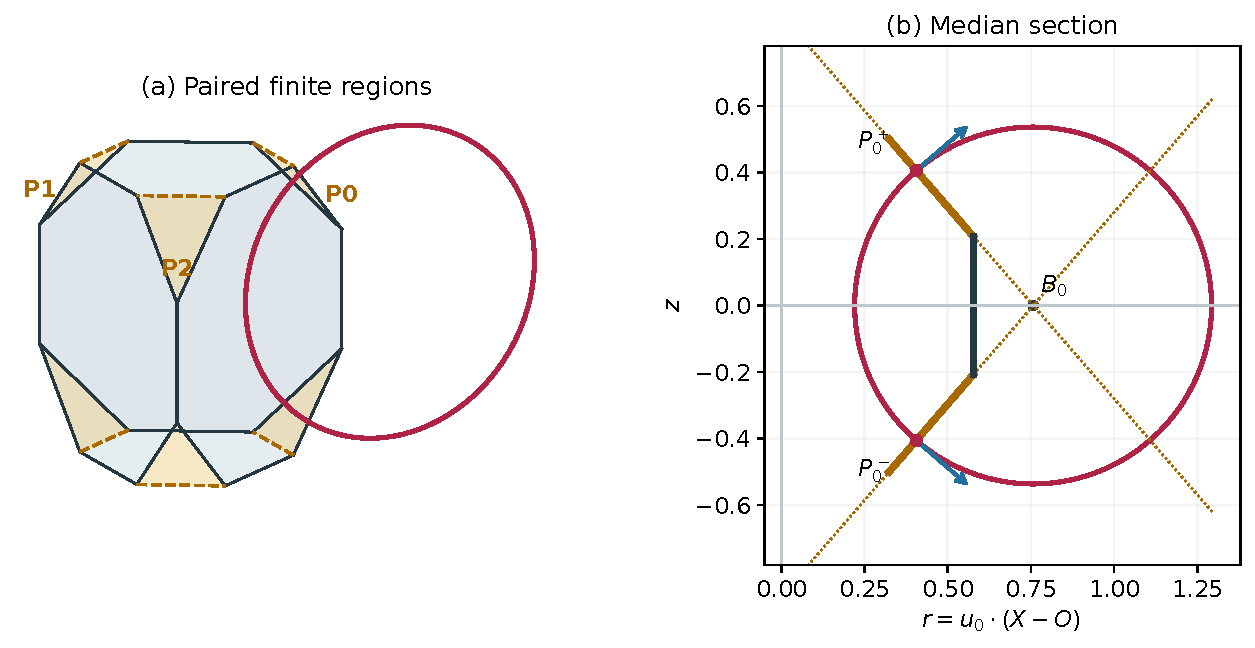
\includegraphics[width=\linewidth]{figures/paired_geometry.pdf}
\caption{Width-one paired geometry and the selected local circle. Left: all material panels and edges, with three upper/lower measurement pairs; dashed gold bases are measurement-only closures. Only $\Gamma_0$ is drawn. Right: its median section, exact interior contacts and patch normals. The blue vectors are geometric normals. The finite measurement segments are distinguished from their dotted supporting lines. Red is a spatial centreline without a time or flow law.}\label{fig:geometry}
\end{figure}

\subsection{A shared point does not establish a shared path}\label{sec:grazing}
The recovered unit frozen macro reference has, near an upper median contact, the curve
\begin{equation}\label{eq:macrocurve}
\mathcal M_j(\nu)=O+a\cos3\nu(\cos\nu\,u_j+\sin\nu\,v_j+\ez).
\end{equation}
At $\nu=0$ it equals $P_j^+$, but $\mathcal M_j'(0)=a v_j$. Its signed plane residual is
\[
f(\nu)=a\cos3\nu(\cos\nu+c)-\kk,\qquad
f(0)=f'(0)=0,\quad f''(0)=-a(10+9c)<0.
\]
Thus it grazes that plane locally, whereas Theorem~\ref{thm:circle} gives a normal crossing. In fact $f\le0$ globally, with equality only at $\nu\in2\pi\mathbb Z$: the product is at most $|\cos\nu+c|\le1+c$, and the latter bound is attained only when $\cos\nu=1$. The other two extrema concern rotated patches, not additional equality points for this fixed patch. This incorporates the later direction-note qualification to the original contact review.~\cite[Sec.~5.4]{GateDirections}

The reference amplitude in \eqref{eq:macrocurve} is a geometric calibration. It is not a supplied native record. For example, the literal staged defaults and $t_c\ge0$ below give $|z_s|\le0.618$; the fixed median scale $a$ would require unit reference amplitude to reach a selected median contact. The construction does not claim that an observed staged point has passed through a patch. Also $M(-z_s)=-M(z_s)$ reverses the horizontal ray as well as height; it is not merely an upper/lower relabelling of a fixed pair.~\cite[Sec.~5.1]{GateDirections}

\subsection{What a tube would add}
One may write the optional family
\begin{equation}\label{eq:tube}
T_j(\chi,\psi;\tau)=B_j+(R_\Gamma+\tau\cos\psi)
(\cos\chi\,u_j+\sin\chi\,\ez)+\tau\sin\psi\,v_j.
\end{equation}
For $0<\tau<R_\Gamma$, the two parameter derivatives are perpendicular with nonzero lengths $R_\Gamma+\tau\cos\psi$ and $\tau$, so this is a regular circular torus. The positive radial factor also gives the usual embedded torus, rather than a spindle self-intersection. Compactness and Theorem~\ref{thm:clearance} imply $\dist(\Gamma_j,S)>0$. The additional sufficient condition $\tau<\dist(\Gamma_j,S)$ makes the tube disjoint from $S$, by the triangle inequality. No numerical thickness or minimum clearance is chosen here. Likewise three possible circles do not choose a physical loop count. A common carrier through all six contacts would require a separately defined nonplanar geometry.

\section{Complete quarter-turned observer modules}\label{sec:placement}
Let $e_r(\phi)=(\cos\phi,\sin\phi,0)$ and $e_\phi(\phi)=(-\sin\phi,\cos\phi,0)$. The recovered Gate/Torus operation is a composition, not just a rotation matrix. First centre a point of the complete shell, then apply
\begin{equation}\label{eq:frames}
Q_x(\pi/2)=\begin{pmatrix}1&0&0\\0&0&-1\\0&1&0\end{pmatrix},\qquad
B(\phi)=[e_r,e_\phi,\ez]Q_x(\pi/2)=[e_r,\ez,-e_\phi].
\end{equation}
Scale the result by $s_m>0$ and translate it to a specified centre. In the original shell coordinates the general ring is
\begin{equation}\label{eq:placement}
\begin{aligned}
\phi_{mk}&=\phi_{m0}+2\pi k/12,& k&=0,\ldots,11,\\
c_{mk}&=O+R_m e_r(\phi_{mk})+h_m\ez,& R_m&>0,\\
X_{mk}(p)&=c_{mk}+s_m B(\phi_{mk})(p-O),&p&\in S.
\end{aligned}
\end{equation}
The local first axis before the moving frame is the quarter-turn axis. Thus $B\ez=-e_\phi$, while $B$ is right-handed orthonormal. Each object is all three filled panels of $S$. Neither a point marker nor a sphere replaces the object; a bounding sphere below is only a clearance tool. The original Gate coordinates put the common centre at zero; adding $O$ in \eqref{eq:placement} expresses the same construction in Paper C coordinates.~\cite[Sec.~6]{Gate}

\begin{proposition}[Sufficient full-module clearances]\label{prop:balls}
Put
\[
B_S=\sqrt{13/12-\sqrt2/2},\qquad \rho_m=s_mB_S.
\]
Within one ring, between two distinct rings, and from each ring to the central shell and every local circle, respectively, sufficient separation conditions are
\begin{equation}\label{eq:bounds}
\begin{aligned}
2R_m\sin(\pi/12)&>2\rho_m,\\
\sqrt{(R_m-R_n)^2+(h_m-h_n)^2}&>\rho_m+\rho_n,\\
\sqrt{R_m^2+h_m^2}&>B_S+\rho_m,\\
\sqrt{R_m^2+h_m^2}&>\kk+R_\Gamma+\rho_m.
\end{aligned}
\end{equation}
These bounds concern filled modules and do not depend on their orientations.
\end{proposition}
\begin{proof}
The panel-centre distance from $O$ is $1/(2\sqrt3)$; the local vertex radius squared is $1/4+h_0^2$. Their perpendicular sum is $B_S^2$. All vertices thus lie in the radius-$B_S$ ball, and convexity places each entire polygon in that ball. A scaled, orthogonally placed copy lies in the radius-$\rho_m$ ball about its centre. On a twelve-site ring, the smallest centre distance is the adjacent chord $2R_m\sin(\pi/12)$. Between rings it is at least the second left side of \eqref{eq:bounds}, because the squared horizontal distance is $(R_m-R_n)^2+2R_mR_n(1-\cos\Delta\phi)$. The shell and each circle are contained in balls about $O$ of radii $B_S$ and $\kk+R_\Gamma$. Subtracting the two enclosing radii from a centre distance proves every claim. The bound is sufficient, not an optimized packing or exact surface distance.
\end{proof}

The H family has five levels $h_2,h_1,0,-h_1,-h_2$, with $0<h_1<h_2$ and freely declared radii, scales and angular origins. The R family has three ordered radii $R_1<R_2<R_3$ at a common height. For the accepted controls, H fixes $R_m=3$, $s_m=1/4$, $h_m\in\{2a,a,0,-a,-2a\}$; R fixes $h_m=0$, $s_m=1/4$, $R_m\in\{2,3,4\}$. Both use $\phi_{m0}=\pi/2$. All bounds in \eqref{eq:bounds} are positive; the smallest fixture margin is $a-B_S/2=0.0988331215\ldots$. These are separate controls. Their 60 and 36 labels total 96, but H0 and the middle R ring are the same twelve sites and frames. Their union has 84 distinct sites. It is not an instantiated height-by-radius product. The combined family remains the parameter list $(R_{\ell r},h_\ell,s_{\ell r},\phi_{\ell r,0})$.

\begin{proposition}[Matched centres are not mirrored bodies]\label{prop:mirror}
For equal radius, scale and angular origin at heights $\pm h$, horizontal reflection interchanges the centres and enclosing balls. Under the same-$B$ convention in \eqref{eq:placement}, it does not interchange the complete miniature shells.
\end{proposition}
\begin{proof}
Let $S_z=\diag(1,1,-1)$. Then $S_zB=B D$, where $D=\diag(1,-1,1)$ acts in the centred source coordinates. Literal reflection of a complete module would therefore require $D(S-O)=S-O$. A seam vertex has centred local $y=\sqrt3/3$; its $D$ image has $y=-\sqrt3/3$, below the minimum centred $y=-\sqrt3/6$ of $S$. Thus this equality fails. The centres and balls still reflect, because the centre heights change sign and a ball is invariant under all orthogonal maps.
\end{proof}

\begin{figure}[htbp]\centering
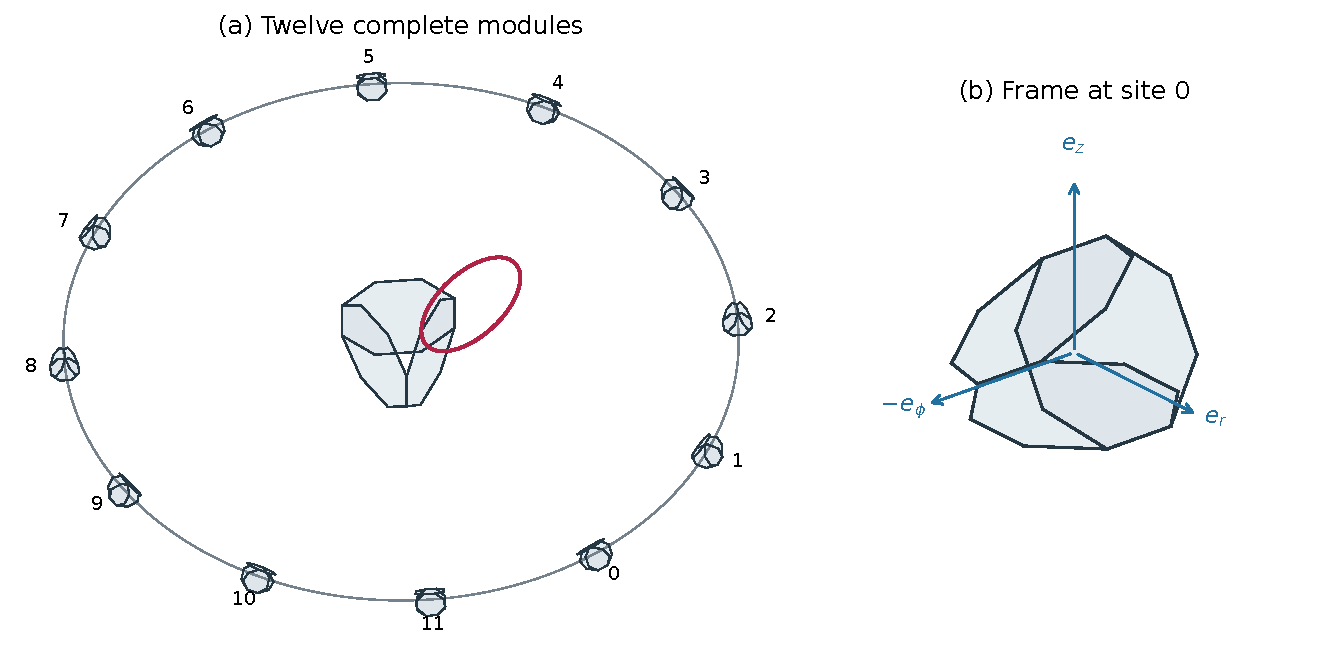
\includegraphics[width=\linewidth]{figures/full_modules.pdf}
\caption{Recovered full-module placement, with $R_c=3$, $s_k=1/4$, $\phi_0=0$. All twelve complete shells are drawn. The inset shows the local orthonormal frame and the original shell axis carried to $-e_\phi$. Grey is the exterior placement circle; red is the separate local $\Gamma_0$. No connecting surface is implied.}\label{fig:modules}
\end{figure}

\begin{figure}[htbp]\centering
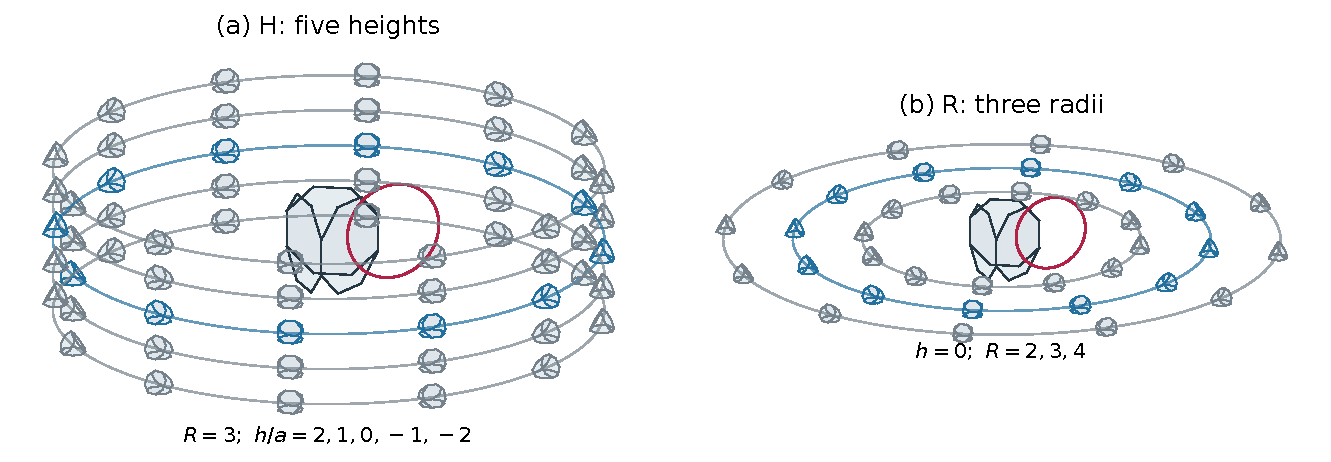
\includegraphics[width=\linewidth]{figures/hr_controls.pdf}
\caption{Separate H and R controls with their prescribed complete modules ($s_m=1/4$, $\phi_{m0}=\pi/2$). H varies height at radius 3; R varies radius at height zero. The common H0/R2 ring is highlighted in blue. Height matching reflects centres and bounding balls, not complete bodies under the same-$B$ convention. No H$\times$R layout is evaluated.}\label{fig:hr}
\end{figure}
